% Author: Dominik Harmim <harmim6@gmail.com>

\documentclass[10pt, xcolor=pdflatex, hyperref={unicode}]{beamer}

\usepackage{newcent}
\usepackage[utf8]{inputenc}
\usepackage[czech]{babel}
\usepackage[T1]{fontenc}
\usepackage{hyperref}
\usepackage{fancyvrb}
\usepackage{graphics}
\usepackage{listings}
\usepackage{xcolor}

\lstset{
	keywordstyle=\color[RGB]{167, 29, 93},
	language=C,
	tabsize=2,
	morekeywords={lock, unlock},
	frame=shadowbox
}


\usetheme{FIT}

\title[
	Statická analýza v~nástroji Facebook Infer zaměřená na detekci
	porušení atomičnosti
]{
	Statická analýza v~nástroji Facebook Infer zaměřená na detekci
	porušení atomičnosti
}

\author[]{\texorpdfstring{
	Dominik Harmim\\
	\small{Vedoucí: Prof. Ing. Tomáš Vojnar, Ph.D.}
}{}}

\institute[]{
	xharmi00@stud.fit.vutbr.cz\\
	Vysoké učení technické v~Brně, Fakulta informačních technologií
}

\date{}


\begin{document}


\frame[plain]{\titlepage}


\begin{frame}[fragile]\frametitle{Motivace}
	\begin{itemize}
		\setlength\itemsep{2em}

		\item
			\important{Atomicita} (provádění operací bez přerušení)

			\begin{itemize}
				\setlength\itemsep{0.5em}

				\item
					je vyžadována v~\emph{paralelních programech},

				\item
					porušení může mít \emph{kritické následky}.
			\end{itemize}
	\end{itemize}

	\begin{columns}
		\begin{column}{0.5 \linewidth}
			\centering
			\begin{lstlisting}
replace(a, b) {
	if (contains(a)) {
		i = index_of(a);
		set(i, b);
	}
}
			\end{lstlisting}
		\end{column}

		\begin{column}{0.5 \linewidth}
			\centering
			\texttt{contains} a~\texttt{index\_of} by měly být
			volány atomicky
		\end{column}
	\end{columns}

	\medskip

	\begin{itemize}
		\setlength\itemsep{2em}

		\item
			\important{Nedostatky současných analyzátorů}
			porušení atomicity:

		\begin{itemize}
			\setlength\itemsep{0.5em}

			\item
				vysoká míra falešných pozitiv,

			\item
				rychlost,

			\item
				škálovatelnost,

			\item
				...
		\end{itemize}
	\end{itemize}
\end{frame}


\begin{frame}[fragile]\frametitle{Facebook Infer}
	\begin{itemize}
		\setlength\itemsep{0.5em}

		\item
			Volně šířený nástroj pro \emph{statickou analýzu}.

		\item
			Používá \important{abstraktní interpretaci (Infer.AI)}.

		\item
			Analýza jednotlivých funkcí od listů stromů ke kořenům.

			\begin{itemize}
				\setlength\itemsep{0.5em}

				\item
					Počítání souhrnů funkcí (\important{summary}).
			\end{itemize}

		\item
			Důraz na \emph{škálovatelnost}.
	\end{itemize}

	\begin{columns}
		\begin{column}{0.3 \linewidth}
			\centering
			\begin{lstlisting}
main() {
	f();
	g();
}
			\end{lstlisting}
		\end{column}

		\begin{column}{0.7 \linewidth}
			\centering
			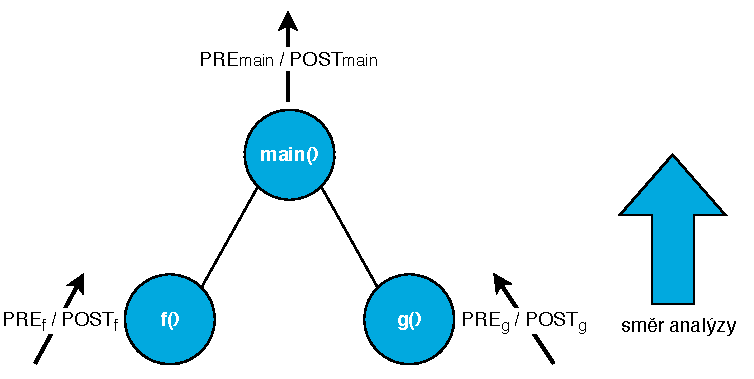
\includegraphics[width=1 \linewidth]{img/infer.pdf}
		\end{column}
	\end{columns}
\end{frame}


\begin{frame}[fragile]\frametitle{Návrh řešení}
	\textbf{Dvě fáze analýzy}:

	\begin{columns}[t]
		\begin{column}{0.5 \linewidth}
			\centering
			\begin{enumerate}
				\item
					\emph{Detekce atomických sekvencí}

					\begin{itemize}
						\setlength\itemsep{0.5em}

						\item
							Derivace množin funkcí volaných
							atomicky.
					\end{itemize}
			\end{enumerate}

			\begin{lstlisting}
f() {
	h1();
	lock();
	h2();
	h3();
	unlock();
	h4();
}
			\end{lstlisting}

			\important{\texttt{
				(h2~h3)~$ \rightarrow $~POST\textsubscript{f}
			}}
		\end{column}

		\begin{column}{0.5 \linewidth}
			\centering
			\begin{enumerate}
				\setcounter{enumi}{1}

				\item
					\emph{Detekce porušení atomicity}

					\begin{itemize}
						\setlength\itemsep{0.5em}

						\item
							Porušení pro libovolnou dvojici, která
							se vyskytla za sebou v~atomické sekvenci
							z~1.~fáze.
					\end{itemize}
			\end{enumerate}

			\begin{lstlisting}
g() {
	h1();
	h2();
	h3();
	h4();
}
			\end{lstlisting}

			\important{Porušení atomicity pro \texttt{h2~h3}.}
		\end{column}
	\end{columns}
\end{frame}


\begin{frame}\frametitle{Shrnutí}
	\textbf{Současný stav:}
	\begin{itemize}
		\setlength\itemsep{0.5em}

		\item
			Implementace \important{detekce atomických sekvencí}
			(1.~fáze).

			\begin{itemize}
				\setlength\itemsep{0.5em}

				\item
					Pro jazyk~\emph{C} se zámky typu
					\emph{POSIX Threads (Pthreads)}.

				\item
					Experimentální ověření.
			\end{itemize}
	\end{itemize}

	\medskip

	\textbf{Budoucí cíle:}
	\begin{itemize}
		\setlength\itemsep{0.5em}

		\item
			Implementace \important{detekce porušení atomicity}
			(2.~fáze).

			\begin{itemize}
				\setlength\itemsep{0.5em}

				\item
					Experimentální ověření.
			\end{itemize}

		\item
			Žádost o~začlenění do repositáře
			\emph{Facebook Infer}
			(\important{Pull~Request}).
	\end{itemize}
\end{frame}


\end{document}
